\documentclass[12pt, a4paper]{article}

\usepackage{amsmath}
\usepackage{graphicx}
%\usepackage{setspace}
%\usepackage[cm]{fullpage}
\usepackage{a4wide}
\usepackage[colorlinks, breaklinks=true, bookmarks=true]{hyperref}

%\doublespacing

%\let\WriteBookmarks\relax

% functions and operations that shouldn't be in Italic font:
\newcommand{\sech}{\mathrm{sech}}
\newcommand{\Real}{\mathrm{Re}}
\newcommand{\Imag}{\mathrm{Im}}
\newcommand{\Tr}{\mathrm{Tr}}

% derivatives:

\newcommand{\deriv}[2]{\frac{d#1}{d#2}}
\newcommand{\nderiv}[3]{\frac{d^#3#1}{{d#2}^#3}}
\newcommand{\pderiv}[2]{\frac{\partial#1}{\partial#2}}
% 2'nd partial derivatives:
\newcommand{\spderiv}[2]{\frac{\partial^2#1}{{\partial#2}^2}}
\newcommand{\pderivdd}[3]{\frac{\partial^2#1}{\partial#2\partial#3}}
% functional derivatives:
\newcommand{\fnlderiv}[2]{\frac{\delta#1}{\delta#2}}
\newcommand{\fnlderivdd}[3]{\frac{\delta^2#1}{\delta#2\delta#3}}

% small matrix:
\newenvironment{bsmatrix}{\left[\begin{smallmatrix}}{\end{smallmatrix}\right]}

% big 0 in a matrix:
\newcommand{\BigFig}[1]{\parbox{12pt}{\Huge #1}}
\newcommand{\BigZero}{\BigFig{0}}
%\newcommand{\ket}[1]{\left|#1\right>}
\newcommand{\bra}[1]{\left<#1\right|}
% an eighenstate:
\newcommand{\eigs}[1]{\left|\varphi_{#1}\right>}
% brackets with operator:
\newcommand{\bracketsO}[3]{\left<#1 \left|#2 \right|#3 \right>}
% with a bigger |:
\newcommand{\bracketsObigm}[3]{\left<#1\! \bigm|\!#2 \!\bigm|\!#3 \right>}
% with the biggest |:
\newcommand{\bracketsObiggm}[3]{\left<#1\! \biggm|\!#2 \!\biggm|\!#3 \right>}
% brackets without operator:
\newcommand{\brackets}[2]{\left<#1 | #2\right>}
% with a bigger |:
\newcommand{\bracketsbigm}[2]{\left<#1 \bigm| #2\right>}
% with the biggest |:
\newcommand{\bracketsbiggm}[2]{\left<#1 \biggm| #2\right>}
% expectation value:
\newcommand{\exval}[1]{\left<#1 \right>}
% bold operator:
\newcommand{\operator}[1]{\mathbf{\hat#1}}
% commutation relation:
\newcommand{\commut}[2]{\left[#1, #2\right]}

\newcommand{\etal}{\textit{et al.}\ }
\newcommand{\ie}{i.\,e.\ }
\newcommand{\eg}{e.\,g.\ }

\begin{document}
\title{Conduction\\
Computational Project No. 1}
\author{Ido Schaefer}
\date{\today}
\maketitle

\section{Trapeze and Simpsom integration}
The Trapeze and the Simpsom integration methods are implemented in the functions \texttt{eq\_space\_trapeze.m} and \texttt{eq\_space\_simpson.m}.

The script files \texttt{test\_trapz.m} and \texttt{test\_simpson.m} demonstrate the error decay of both methods, where $\log_{10}(Error)$ is plotted Vs.\ $\log_{10}N$. The integrated function in \texttt{test\_trapz.m} is $f(x)=x^2$. The integrated function in \texttt{test\_simpson.m} is $f(x)=\sin(x)$. The resulting curves are shown in Figs.~\ref{fig:trapeze}, \ref{fig:simpson}. The resulting curves were fitted to a linear form. The slope for the Trapeze method is $-2$, and for the Simpson method is $-4$, as expected.

\begin{figure}[htb]
	\centering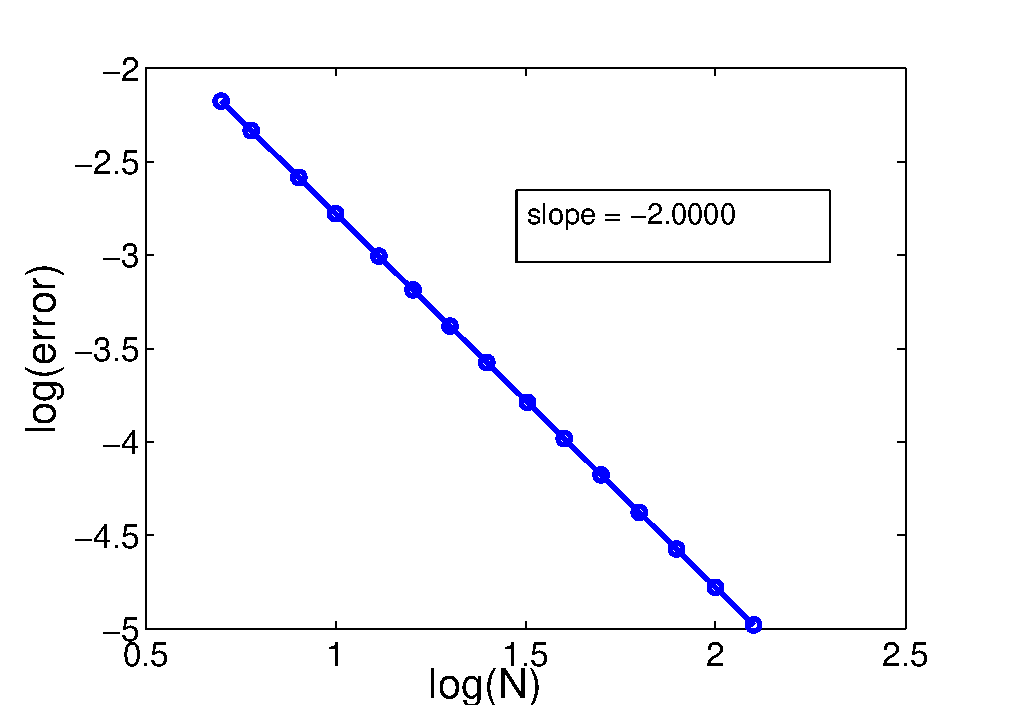
\includegraphics[width=3in]{trapeze}
	\caption{Error decay curve for the Trapeze method}\label{fig:trapeze}
\end{figure}

\begin{figure}[htb]
	\centering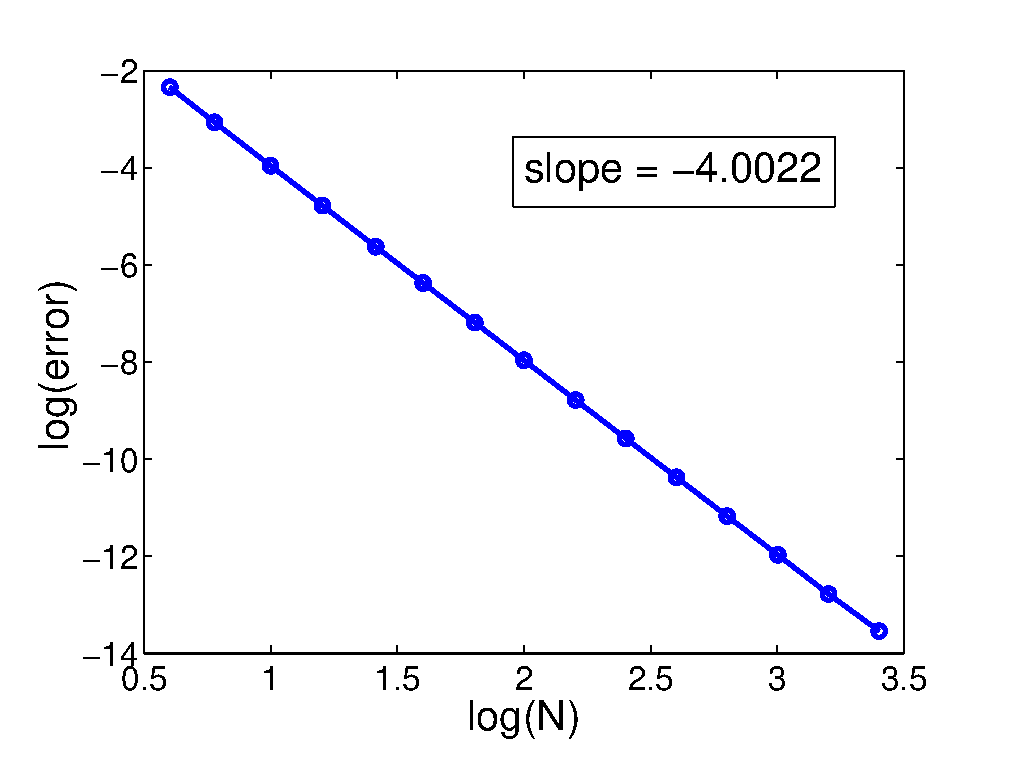
\includegraphics[width=3in]{simpson}
	\caption{Error decay curve for the Simpson method}\label{fig:simpson}
\end{figure}

\section{Transfer probability computation}
The procedure \texttt{trans\_coef.m} computes $T(E)$ for a given $E$. The procedure \texttt{getTv.m} computes the function $T(E)$ for a given range of energies using \texttt{trans\_coef.m}.

\section{Computation of $T(E)$ for two systems}
The implementation of \texttt{trans\_coef.m} is demonstrated in the procedures \texttt{rect\_barrier.m} and \texttt{periodic\_barrier.m}, for the systems requested in part 3 of the project.

The expected result for a classical particle in both systems is a transfer of the particle with $E$ above the hight of the barrier (\text{$W=10_{eV}$} or \text{$W_0=8_{eV}$}), and no transfer with $E$ below it.

The resulting curve for the rectangular barrier is shown in Fig.~\ref{fig:rectb}. It can be seen that there is small transfer also below $W$, due to a tunnelling effect. $T(E)$ grows sharply in the region of \text{$E=W$}, in accordance with the classical picture. However, unlike in the classical picture, $T(E)$ continues to oscillate in the region of \text{$E>W$}, with maxima of \text{$T(E)=1$}. The amplitude of these oscillations decreases with $E$, and the ``wavelength'' increases. Thus, the picture is getting more similar to the classical picture. These oscillations demonstrate that in the quantum picture, the transfer probability is affected by the coincidence with the quantized resonance frequencies of the system, and not only by energy considerations.

\begin{figure}[htb]
	\centering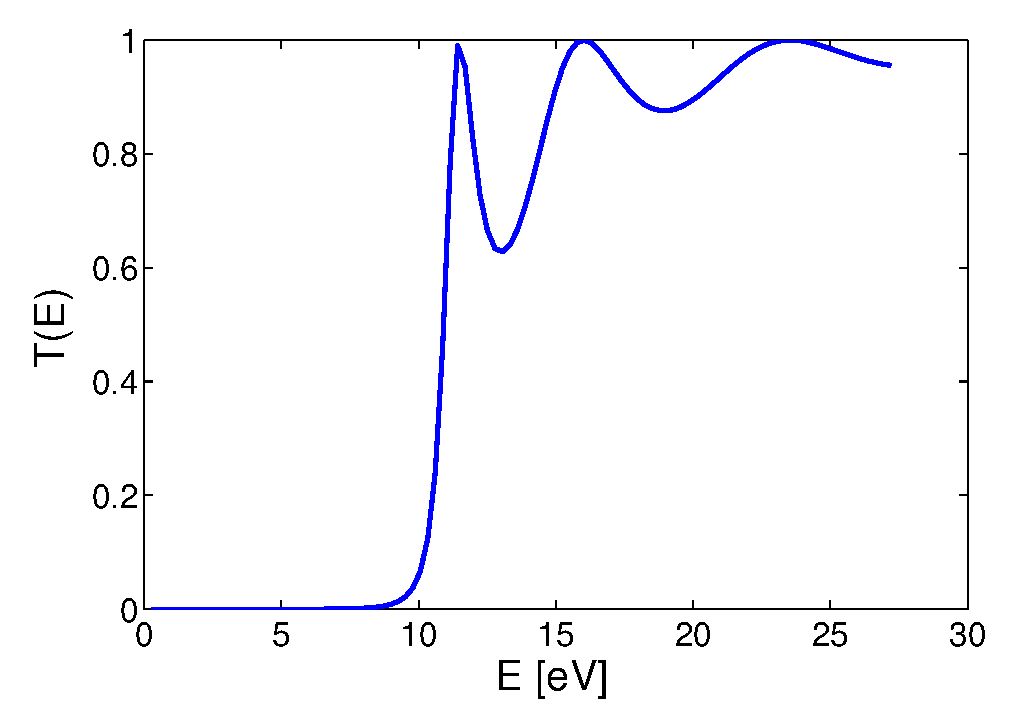
\includegraphics[width=3in]{rect_barrier}
	\caption{$T(E)$ for the rectangular barrier system}\label{fig:rectb}
\end{figure}

The resulting curve for the periodic barrier is shown in Fig.~\ref{fig:periodicb}. Here the picture deviates appreciably from the classical picture. There is a large and broad resonance below $W_0$, which decays almost to $0$ in the region of \text{$E=W_0$}. Probably, the periodic structure has a similar effect to the double-barrier effect, where there is a large transfer when $E$ coincides with one of the resonances of the double-barrier. Here, the maximum is much broader. In larger energies, the picture becomes similar to that of the rectangular barrier, and thus to the classical picture.

\begin{figure}[htb]
	\centering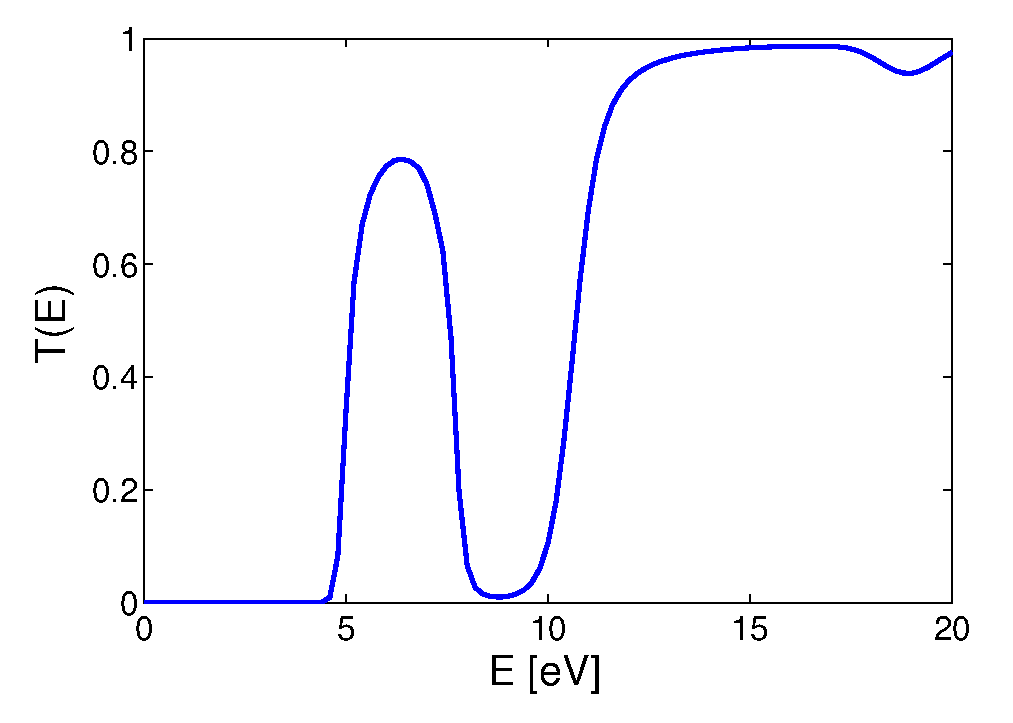
\includegraphics[width=3in]{periodic_barrier}
	\caption{$T(E)$ for the periodic barrier system}\label{fig:periodicb}
\end{figure}

\section{Double barrier system}
\subsection{Computation of $T(E)$, analysis, and variation of the parameters}
$T(E)$ for the double barrier problem is computed in the procedure \texttt{double\_barrier.m} (with $V_g=0$). The resulting curve is shown in Fig.~\ref{fig:doubleb}.

There are several resonances at energies lower than the barrier hight, \text{$W_L=W_R=10_{eV}$}. A resonance should occur in an energy that coincides with the energy of one of the ``bound states'' of the double barrier.

\begin{figure}[htb]
	\centering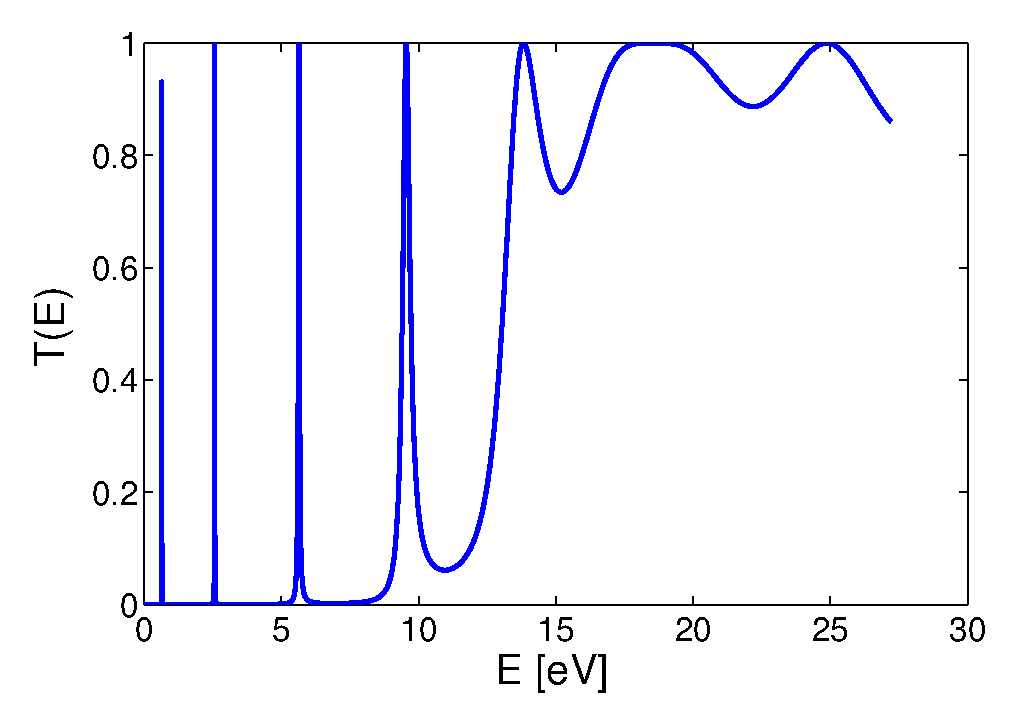
\includegraphics[width=3in]{double_barrier}
	\caption{$T(E)$ for the double barrier system}\label{fig:doubleb}
\end{figure}

The effect of the variation of the various parameters was tested. When $W$ is increased, the resonance energies become higher, and are getting closer to these of a particle in a box:
\begin{equation}\label{eq:box}
	E_n = \frac{n^2\pi^2\hbar^2}{2mL^2}
\end{equation}
This can be readily explained by the fact that the double barrier system is getting closer to a double infinite potential well. The resonances are getting narrower. A possible explanation is that the ``lifetime'' of the bound states in the double-barrier is longer, because the increment of the barrier hight decreases the tunnelling rate. Thus, the energy levels are sharper, due to the Heisenberg uncertainty principle. A decrement of $W$ has the opposite effect. The resonance energies are getting lower and denser, especially the energies that are close to $W$. This is a well known effect also in other systems with a finite well.

The increment of $L$ has the effect of lowering the resonance energies. The energy levels are getting denser. This result could be expected from Eq.~\eqref{eq:box}.

The increment of $D$ decreases the width of the resonances. The explanation can be similar to that of the same effect when $W$ is increased. Another effect is a slight increment of the resonance energies corresponding to the bound states. This can be explained by the fact that ``passing over'' a wider energy barrier is in a greater contradiction to the classical picture, and hence more difficult. The ``bound-states'' of the well become more ``bound'', and the particle-in-a-box model becomes more appropriate. In contrary to the resonance energies of the bound states, the resonance energies above $W$ become lower.

The increment of $V_g$ has the effect of a corresponding increment of the resonance energies, as could be expected from the particle-in-a-box model. The energy levels near the threshold of the well are getting denser.

\subsection{Computation of $I(V)$}
$I(V)$ is computed in the procedure \texttt{I\_V.m}. The temperature is chosen to be \text{$T=298^{\circ}K$}. After some algebra, one finds that the difference of $F_D$ between the electrodes is given by the expression:
\begin{equation}\label{eq:DeltaF}
	\Delta F_D = \frac{\sinh\left(\frac{\beta eV}{2}\right)}{\cosh\left(\frac{\beta eV}{2}\right) + \cosh[\beta(E-\mu)]}
\end{equation}
This expression is used in the procedure. The integral is computed by the Simpson method.

The resulting curve is shown in Fig.~\ref{fig:I_V}. There are ``jumps'' in $I(V)$ around $V=1.29_V$ and $V=4.87_V$. These jumps can be explained by the examination of the dependence of the integrand on $V$. $T(E)$ is independent of $V$. The $V$ dependence is contained in the function $\Delta F_D$. This function may be viewed as a ``window'' of the energy range which contributes to the current. This window is getting wider as $V$ increases. In the neighbourhood of a $V$ value in which a resonance energy is absorbed in the energy window, there will be a jump in $I(V)$. This explanation can be verified by examining the shape of $\Delta F_D$ in the relevant $V$ values. In Fig.~\ref{fig:jumps}, $T(E)$ and $\Delta F_D$ for the relevant $V$ values are plotted Vs.\ $E$. It can be seen that a resonance energy in $T(E)$ is absorbed into the window in each of the ``jumps'' in $I(V)$.

\begin{figure}[htb]
	\centering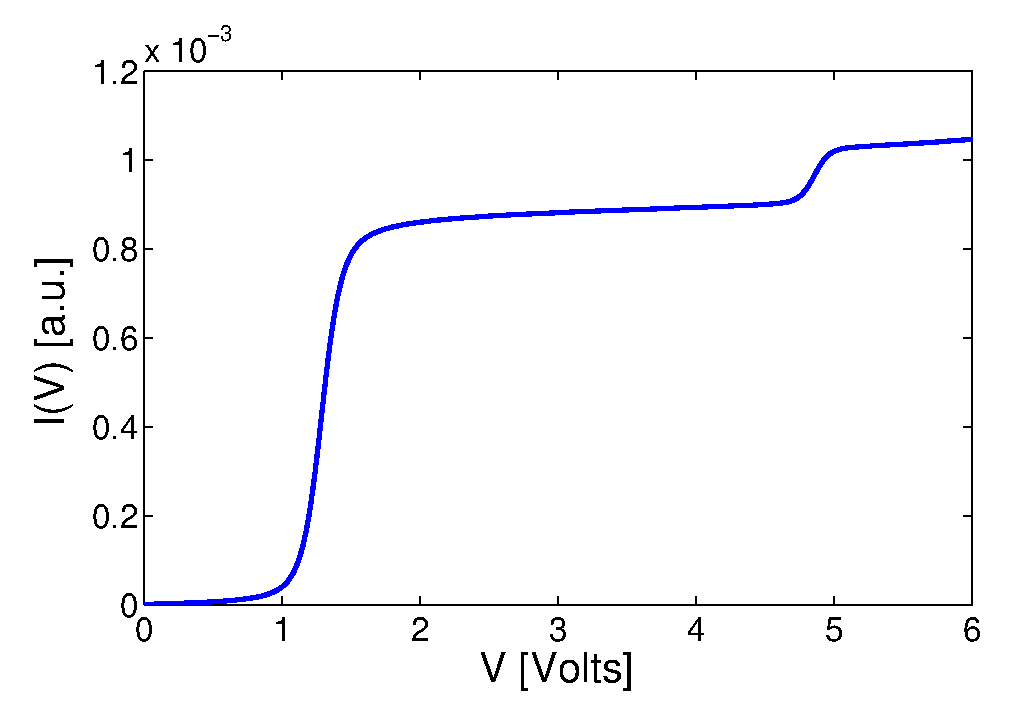
\includegraphics[width=3in]{I_V}
	\caption{$I(V)$ for the double barrier system}\label{fig:I_V}
\end{figure}

\begin{figure}[htb]
	\centering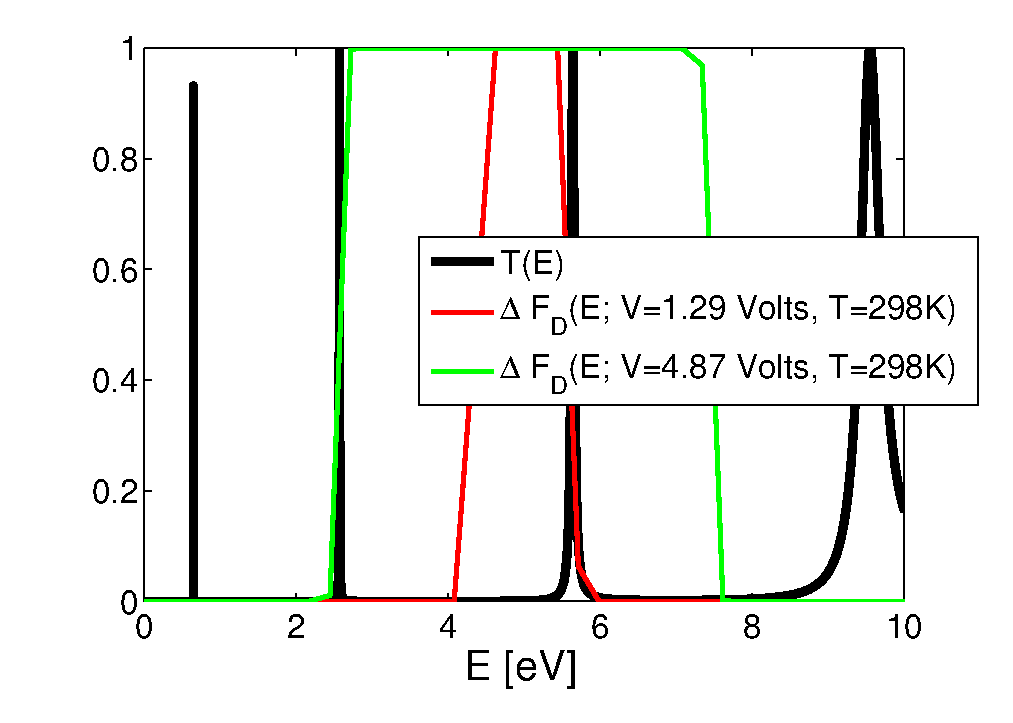
\includegraphics[width=3in]{current_jumps}
	\caption{$T(E)$ and $\Delta F_D$ in the $V$ values in which a ``jump'' in $I(V)$ occurs, are plotted Vs.\ $E$.}\label{fig:jumps}
\end{figure}

It can be also deduced from Fig.~\ref{fig:jumps} which ``jump'' corresponds to an electron flow, and which to a hole flow. The resonance energy absorbed in the neighbourhood of $V=1.29_V$ is higher than the Fermi level, $\mu=5_{eV}$. Thus, this jump originates from an electron flow. The resonance energy absorbed in the neighbourhood of the jump in $V=4.87_V$ is lower than the Fermi level, and thus, corresponds to a hole flow. 

\subsection{Computation of the conduction}
The conduction is given by:
\begin{equation}\label{eq:g}
	g(V, V_g) = \deriv{I}{V} = \frac{2e}{h}\int_0^\infty \deriv{\Delta F_D(E, V)}{V}T(E, V_g)\,dE
\end{equation}
Taking the derivative of $\Delta F_D$ with respect to $V$ we obtain:
\begin{equation}\label{eq:dDeltaFdV}
	\deriv{\Delta F_D}{V}= \frac{\beta e}{2}\frac{\cosh\left(\frac{\beta eV}{2}\right) \cosh[\beta(E-\mu)] + 1}{\left\lbrace \cosh[\beta(E-\mu)] + \cosh\left(\frac{\beta eV}{2}\right) \right\rbrace^2}
\end{equation}

In the procedure \texttt{conduction.m}, $g(V, V_g)$ is computed and plotted Vs.\ $V$ and $V_g$ for the range \text{$0<V\leq 6$}, \text{$-3\leq V_g\leq 3$}. The resulting surface is shown in Fig.~\ref{fig:g}. The resulting shape is similar to that of the experimental results (Fig.~3 in the article).

The peaks in $g(V, V_g)$ correspond to the jumps in $I(V)$, and hence, indicate the absorption of a resonance by the energy window $\Delta F_D$. The function $\Delta F_D$ is symmetric around $\mu$ with respect to $E$ (see Eq.~\eqref{eq:DeltaF}), and the width of the window grows with $V$. Thus, a shift of the resonance energies will have a different effect on the position of the peaks in $g(V)$ with respect to $V$, for different resonances. For a resonance energy higher than the Fermi level ($E_{res}>\mu$), a positive shift will shift the peaks of $g(V)$ in the positive direction. For a resonance energy lower than the Fermi level ($E_{res}<\mu$), a positive shift will shift the peaks of $g(V)$ in the negative direction. A positive shift of $V_g$ causes a positive shift of the resonance energies in $T(E)$. In Fig.~\ref{fig:g}, we see that for each of the resonances, there are two nearly strait-line branches splitting from $V=0_V$, one with a positive slope, for $E_{res}>\mu$, and one with a negative slope, for $E_{res}<\mu$.

In the case of $E_{res}>\mu$, the resonance level in the junction is above the Fermi level, and hence is unoccupied. Thus, the current consists of an electron flow. In the case of $E_{res}<\mu$, the resonance level in the junction is occupied, and the current consists of a hole flow.

\begin{figure}[htb]
	\centering\includegraphics[width=3in]{conduction1}
	\caption{$g(V, V_g)$ is plotted Vs.\ $V$ and $V_g$.}\label{fig:g}
\end{figure}


\end{document}